\documentclass[conference]{IEEEtran}
\IEEEoverridecommandlockouts
\usepackage[utf8]{inputenc}
\usepackage[T1]{fontenc}
\usepackage[spanish,es-tabla,es-nodecimaldot]{babel}
\usepackage{cite}
\usepackage{amsmath,amssymb,amsfonts}
\usepackage{graphicx}
\usepackage{textcomp}
\usepackage{xcolor}
\usepackage{url}

\begin{document}

\title{Clasificaci\'on de COVID-19 a partir del sonido de la tos mediante caracter\'isticas MFCC y modelos cl\'asicos de aprendizaje autom\'atico}

\author{%
\begin{tabular}{@{}c@{\hspace{3em}}c@{}}
\shortstack{Roger Re\'ategui Soto\\[.25em]
\textit{Maestr\'ia en DS/AI}\\
\textit{Universidad de Ingenier\'ia y Tecnolog\'ia (UTEC)}\\
Lima, Per\'u}
&
\shortstack{Erick Rosas Pisfil\\[.25em]
\textit{Maestr\'ia en DS/AI}\\
\textit{Universidad de Ingenier\'ia y Tecnolog\'ia (UTEC)}\\
Lima, Per\'u}
\\[1.4em]
\multicolumn{2}{c}{\shortstack{Yemar Puma Huam\'an\\[.25em]
\textit{Maestr\'ia en DS/AI}\\
\textit{Universidad de Ingenier\'ia y Tecnolog\'ia (UTEC)}\\
Lima, Per\'u}}
\end{tabular}%
}

\maketitle

\begin{abstract}
Este trabajo aborda la clasificaci\'on de pacientes como COVID-19 positivos o negativos empleando \'unicamente el sonido de su tos. A partir de las colecciones COSWARA y Virufy, con 1207 toses negativas y 150 positivas, cada grabaci\'on se representa con coeficientes cepstrales en las frecuencias de Mel (MFCC), resumidos mediante su media y desviaci\'on est\'andar. Se comparan cuatro modelos cl\'asicos (Regresi\'on Log\'istica, M\'aquinas de Vectores de Soporte, \'Arbol de Decisi\'on y K vecinos m\'as cercanos) y, adicionalmente, Random Forest, entrenados con validaci\'on cruzada de cinco particiones a nivel de paciente para evitar la fuga de datos. Dado el fuerte desbalance de clases (89/11), la evaluaci\'on prioriza el F1 y el recall de la clase positiva. El mejor modelo fue una SVM con kernel RBF. Se estudiaron varias estrategias de mejora; el ajuste del umbral de decisi\'on result\'o la m\'as efectiva, elevando el recall de positivos de 0.42 a 0.50 y la exactitud balanceada de 0.69 a 0.72 en el conjunto de prueba, con una p\'erdida m\'inima de exactitud global.
\end{abstract}

\begin{IEEEkeywords}
COVID-19, clasificaci\'on de audio, MFCC, SVM, clases desbalanceadas, validaci\'on cruzada
\end{IEEEkeywords}

\section{Introducci\'on}
La detecci\'on temprana y de bajo costo de infecciones respiratorias es un problema de gran inter\'es. La tos es un s\'intoma frecuente de la COVID-19 y puede registrarse con un simple micr\'ofono, lo que motiva el estudio de sistemas capaces de estimar el riesgo a partir de su sonido. El objetivo de este proyecto es clasificar pacientes como positivos o negativos usando exclusivamente el audio de la tos, aplicando los modelos de clasificaci\'on vistos en el curso.

Las contribuciones de este trabajo son: (i) un flujo de preprocesamiento y extracci\'on de caracter\'isticas basado en MFCC; (ii) una comparaci\'on sistem\'atica de cinco clasificadores mediante validaci\'on cruzada a nivel de paciente; y (iii) un an\'alisis de estrategias para mejorar la detecci\'on de la clase minoritaria, que es la de mayor inter\'es cl\'inico. El c\'odigo y los resultados son reproducibles y est\'an disponibles en el repositorio del proyecto\footnote{C\'odigo: \url{https://github.com/erosas-utec/ml-project-classification} --- Demo web: \url{https://ml-project-classification.onrender.com}}, con una semilla fija.

\section{Conjunto de datos}
El conjunto de datos se construye a partir de muestras de las colecciones COSWARA \cite{coswara} y Virufy \cite{virufy}. Contiene 1207 toses de personas con prueba negativa y 150 de personas positivas. La clase positiva mezcla dos formatos: 102 archivos \texttt{.wav} y 48 \texttt{.mp3}, todos conservados. Existe adem\'as una carpeta \texttt{Unknown} sin etiqueta, que se descarta por no aportar a la medici\'on de m\'etricas.

El conjunto presenta un fuerte desbalance: aproximadamente 89\% de ejemplos negativos frente a 11\% positivos (Fig.~\ref{fig:dist}). Este desbalance condiciona toda la evaluaci\'on, ya que un clasificador que prediga siempre la clase negativa alcanzar\'ia cerca de 89\% de exactitud sin detectar ning\'un caso de COVID-19.

Durante la revisi\'on se identificaron varios detalles de calidad de datos. La etiqueta se toma de la carpeta y no del nombre del archivo, pues nueve archivos presentan el error tipogr\'afico \emph{Postive}. La edad y el g\'enero, incluidos en el nombre de cada archivo, se conservan solo como metadatos descriptivos y no se usan como caracter\'isticas, ya que el objetivo es clasificar \'unicamente con el sonido. Finalmente, cinco pacientes positivos aportan varias grabaciones (por ejemplo, un paciente aporta 22 audios); se verific\'o que son grabaciones distintas y no copias, por lo que se conservan, con la precauci\'on descrita en la Secci\'on~\ref{sec:val}.

\begin{figure}[t]
\centerline{
\includegraphics[width=0.72\columnwidth]{figures/distribucion_clases.png}}
\caption{Distribuci\'on de clases. El conjunto est\'a fuertemente desbalanceado hacia la clase negativa.}
\label{fig:dist}
\end{figure}

\section{Metodolog\'ia}

\subsection{Extracci\'on de caracter\'isticas}
Un audio en crudo es una se\~nal larga y de duraci\'on variable (entre 2.5 y 26 segundos), por lo que no puede utilizarse directamente como entrada de los modelos. El enunciado permite emplear librer\'ias para obtener el mejor vector de caracter\'isticas; se utilizan los MFCC \cite{mfcc}, que resumen el timbre del sonido en pocas dimensiones y son un est\'andar en el an\'alisis de audio. La extracci\'on se realiza con la librer\'ia \texttt{librosa} \cite{librosa}.

Para cada audio se calcula la matriz de 20 MFCC por ventana temporal y se resume con la media y la desviaci\'on est\'andar de cada coeficiente, obteniendo un vector fijo de 40 caracter\'isticas, con independencia de la duraci\'on. Adem\'as, la carga remuestrea todas las se\~nales a 22\,050 Hz, lo que unifica los audios que llegan en 44.1 kHz y 48 kHz. Las caracter\'isticas se almacenan en disco para garantizar la reproducibilidad sin necesidad de reprocesar el audio.

\subsection{Partici\'on y escalado}
\label{sec:val}
Se reserva el 20\% de los datos como conjunto de prueba, de forma estratificada y \emph{a nivel de paciente}: primero se reparten los pacientes y luego se asignan sus grabaciones. As\'i, todas las grabaciones de un mismo paciente permanecen en el mismo subconjunto; de lo contrario, el modelo podr\'ia reconocer al paciente en la prueba y las m\'etricas resultar\'ian infladas por fuga de datos. El conjunto de entrenamiento resultante tiene 1067 audios (9.6\% positivos) y el de prueba 290 audios (16.6\% positivos). Las caracter\'isticas se estandarizan con un \texttt{StandardScaler} ajustado \'unicamente con el entrenamiento.

\subsection{Modelos}
Se comparan los cuatro modelos solicitados y un m\'etodo adicional, todos vistos en el curso:
Regresi\'on Log\'istica, que aplica la funci\'on sigmoide sobre una combinaci\'on lineal de las caracter\'isticas;
SVM \cite{svm}, que busca el hiperplano de m\'aximo margen, empleando kernels lineal y RBF;
\'Arbol de Decisi\'on, que particiona el espacio reduciendo la impureza (Gini o entrop\'ia);
K vecinos m\'as cercanos (KNN), que clasifica por votaci\'on de los vecinos;
y Random Forest, un ensamble por \emph{bagging} de \'arboles, incluido como m\'etodo adicional.

\subsection{Validaci\'on y m\'etricas}
La selecci\'on de hiperpar\'ametros se realiza sobre el entrenamiento mediante validaci\'on cruzada de cinco particiones con \texttt{StratifiedGroupKFold}: estratificada, para mantener la proporci\'on de clases en cada partici\'on, y agrupada, para que las grabaciones de un mismo paciente no se repartan entre particiones. Para cada configuraci\'on se reportan exactitud (Acc), exactitud balanceada (BAcc) y precisi\'on (Prec), recall (Rec) y F1 de la clase positiva. Dado el desbalance, el F1 de la clase positiva es la m\'etrica de selecci\'on \cite{scikit}.

\section{Experimentos y resultados}

\subsection{B\'usqueda de hiperpar\'ametros}
Las Tablas~\ref{tab:lr}--\ref{tab:rf} presentan, para cada modelo, las m\'etricas promedio de validaci\'on cruzada por cada configuraci\'on de hiperpar\'ametros probada. Se observa un patr\'on com\'un: casi todas las configuraciones alcanzan una exactitud alta (cercana a 0.90) que proviene de acertar en la clase mayoritaria, mientras que el recall de la clase positiva permanece bajo.

\begin{table}[t]
\caption{Regresi\'on Log\'istica}
\label{tab:lr}
\centering\footnotesize
\begin{tabular}{cccccc}
\hline
$C$ & Acc & BAcc & Prec & Rec & F1 \\
\hline
0.1 & 0.903 & 0.521 & 0.433 & 0.049 & 0.087 \\
1.0 & 0.900 & 0.537 & 0.399 & 0.089 & \textbf{0.142} \\
10  & 0.897 & 0.535 & 0.366 & 0.089 & 0.139 \\
\hline
\end{tabular}
\end{table}

\begin{table}[t]
\caption{SVM (kernel y margen suave $C$)}
\label{tab:svm}
\centering\footnotesize
\begin{tabular}{ccccccc}
\hline
Kernel & $C$ & Acc & BAcc & Prec & Rec & F1 \\
\hline
lineal & 0.1 & 0.904 & 0.500 & 0.000 & 0.000 & 0.000 \\
lineal & 1.0 & 0.904 & 0.500 & 0.000 & 0.000 & 0.000 \\
lineal & 10  & 0.904 & 0.500 & 0.000 & 0.000 & 0.000 \\
RBF    & 0.1 & 0.904 & 0.500 & 0.000 & 0.000 & 0.000 \\
RBF    & 1.0 & 0.910 & 0.530 & 0.800 & 0.060 & 0.110 \\
RBF    & 10  & 0.905 & 0.615 & 0.522 & 0.255 & \textbf{0.339} \\
\hline
\end{tabular}
\end{table}

\begin{table}[t]
\caption{\'Arbol de Decisi\'on (criterio y profundidad)}
\label{tab:dt}
\centering\footnotesize
\begin{tabular}{ccccccc}
\hline
Criterio & Prof. & Acc & BAcc & Prec & Rec & F1 \\
\hline
Gini    & 3    & 0.900 & 0.511 & 0.167 & 0.030 & 0.051 \\
Gini    & 5    & 0.895 & 0.548 & 0.344 & 0.118 & 0.172 \\
Gini    & 10   & 0.868 & 0.555 & 0.218 & 0.169 & 0.190 \\
Gini    & --   & 0.858 & 0.581 & 0.229 & 0.238 & \textbf{0.233} \\
Entrop. & 3    & 0.899 & 0.527 & 0.333 & 0.068 & 0.100 \\
Entrop. & 5    & 0.879 & 0.552 & 0.283 & 0.147 & 0.192 \\
Entrop. & 10   & 0.850 & 0.567 & 0.216 & 0.216 & 0.214 \\
Entrop. & --   & 0.839 & 0.569 & 0.203 & 0.236 & 0.218 \\
\hline
\end{tabular}
\end{table}

\begin{table}[t]
\caption{KNN (vecinos $K$ y ponderaci\'on)}
\label{tab:knn}
\centering\footnotesize
\begin{tabular}{ccccccc}
\hline
$K$ & Peso & Acc & BAcc & Prec & Rec & F1 \\
\hline
3  & uniforme  & 0.906 & 0.588 & 0.531 & 0.195 & \textbf{0.283} \\
3  & distancia & 0.906 & 0.588 & 0.531 & 0.195 & 0.283 \\
5  & uniforme  & 0.913 & 0.570 & 0.730 & 0.147 & 0.242 \\
5  & distancia & 0.914 & 0.575 & 0.750 & 0.157 & 0.256 \\
7  & uniforme  & 0.912 & 0.548 & 0.833 & 0.098 & 0.174 \\
7  & distancia & 0.915 & 0.558 & 0.933 & 0.117 & 0.206 \\
11 & uniforme  & 0.907 & 0.515 & 0.600 & 0.029 & 0.055 \\
11 & distancia & 0.908 & 0.520 & 0.800 & 0.039 & 0.074 \\
\hline
\end{tabular}
\end{table}

\begin{table}[t]
\caption{Random Forest (\'arboles y profundidad)}
\label{tab:rf}
\centering\footnotesize
\begin{tabular}{ccccccc}
\hline
\'Arboles & Prof. & Acc & BAcc & Prec & Rec & F1 \\
\hline
100 & 5  & 0.906 & 0.510 & 0.400 & 0.020 & 0.038 \\
100 & 10 & 0.906 & 0.514 & 0.400 & 0.030 & 0.055 \\
100 & -- & 0.907 & 0.519 & 0.600 & 0.040 & 0.074 \\
200 & 5  & 0.906 & 0.510 & 0.400 & 0.020 & 0.038 \\
200 & 10 & 0.907 & 0.515 & 0.400 & 0.030 & 0.055 \\
200 & -- & 0.908 & 0.520 & 0.600 & 0.040 & \textbf{0.074} \\
\hline
\end{tabular}
\end{table}

\subsection{Comparaci\'on entre modelos}
La Fig.~\ref{fig:comp} compara la mejor configuraci\'on de cada modelo. El mejor F1 de la clase positiva lo obtiene la SVM con kernel RBF y $C=10$ (F1 = 0.339, BAcc = 0.615), seguida de KNN (0.283) y el \'Arbol de Decisi\'on (0.233). Es notable el caso de Random Forest: alcanza la mayor exactitud (0.908) pero un recall de apenas 0.04, es decir, casi no detecta positivos. Este contraste confirma que la exactitud no es una m\'etrica adecuada bajo desbalance y justifica la elecci\'on del F1 de la clase positiva como criterio.

\begin{figure}[t]
\centerline{
\includegraphics[width=\columnwidth]{figures/comparacion_modelos.png}}
\caption{Comparaci\'on de la mejor configuraci\'on de cada modelo (promedio de validaci\'on cruzada). La exactitud es alta en todos, pero el recall de la clase positiva es bajo.}
\label{fig:comp}
\end{figure}

\subsection{Estrategias de mejora}
Partiendo del mejor modelo (SVM RBF), se evaluaron cuatro estrategias, todas con la misma validaci\'on cruzada. La reducci\'on de dimensionalidad con PCA (30 componentes que explican el 95\% de la varianza) y con LDA no mejor\'o el F1 (0.336 y 0.210, frente a 0.339 con los 40 MFCC). La ponderaci\'on de clases (\texttt{class\_weight=balanced}) tampoco lo mejor\'o (0.322), como se resume en la Tabla~\ref{tab:mejoras}, ni el uso de deltas de MFCC de primer y segundo orden (120 caracter\'isticas, F1 = 0.233). Estas estrategias se documentan como exploraci\'on y no se incorporan al modelo final.

\begin{table}[t]
\caption{F1 de la clase positiva (validaci\'on cruzada) de las estrategias exploradas, sobre la SVM RBF}
\label{tab:mejoras}
\centering\footnotesize
\begin{tabular}{lc}
\hline
Estrategia & F1 \\
\hline
MFCC (40), l\'inea base            & \textbf{0.339} \\
PCA (30 componentes)             & 0.336 \\
LDA (1 componente)               & 0.210 \\
Ponderaci\'on de clases           & 0.322 \\
MFCC + deltas (120)              & 0.233 \\
\hline
\end{tabular}
\end{table}

La estrategia efectiva fue el ajuste del umbral de decisi\'on. Los modelos probabil\'isticos deciden por defecto con el umbral 0.5; bajo desbalance, ese valor no es \'optimo para detectar la clase minoritaria. Se obtuvieron las probabilidades fuera de muestra con validaci\'on cruzada y se seleccion\'o el umbral que maximiza el F1 de la clase positiva (Fig.~\ref{fig:umbral}), resultando en 0.25.

\begin{figure}[t]
\centerline{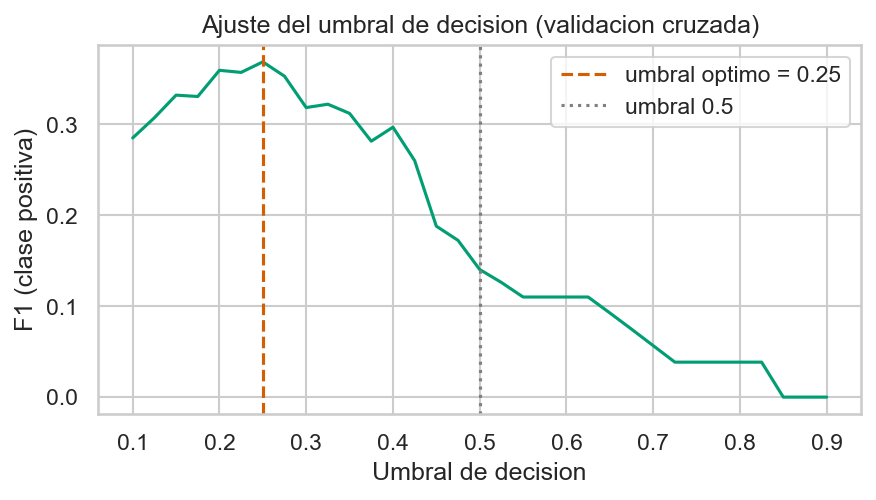
\includegraphics[width=0.85\columnwidth]{figures/umbral.png}}
\caption{F1 de la clase positiva en funci\'on del umbral de decisi\'on (validaci\'on cruzada). El \'optimo (0.25) mejora claramente respecto al umbral por defecto 0.5.}
\label{fig:umbral}
\end{figure}

\subsection{Evaluaci\'on final en el conjunto de prueba}
El modelo final (SVM RBF, $C=10$, con umbral 0.25) se entrena con todo el conjunto de entrenamiento y se eval\'ua una \'unica vez sobre el conjunto de prueba. La Tabla~\ref{tab:test} compara la l\'inea base (umbral 0.5) con el modelo mejorado. El ajuste del umbral eleva el recall de positivos de 0.417 a 0.500, el F1 de 0.533 a 0.558 y la exactitud balanceada de 0.694 a 0.721, con una ca\'ida m\'inima de la exactitud global (de 0.879 a 0.869).

\begin{table}[t]
\caption{Resultados en el conjunto de prueba (m\'etricas de la clase positiva)}
\label{tab:test}
\centering\footnotesize
\begin{tabular}{lccccc}
\hline
Modelo & Acc & BAcc & Prec & Rec & F1 \\
\hline
L\'inea base (umbral 0.5) & \textbf{0.879} & 0.694 & \textbf{0.741} & 0.417 & 0.533 \\
Mejorado (umbral 0.25)   & 0.869 & \textbf{0.721} & 0.632 & \textbf{0.500} & \textbf{0.558} \\
\hline
\end{tabular}
\end{table}

La matriz de confusi\'on del modelo mejorado (Fig.~\ref{fig:cm}) muestra que se detectan 24 de los 48 casos positivos (50.0\%) y se clasifican correctamente 228 de los 242 negativos (94.2\%). La exactitud total es de 0.869. El sistema es, por tanto, m\'as \'util para descartar la enfermedad que para confirmarla, lo cual es coherente con la dificultad de la tarea y con el uso exclusivo del sonido.

\begin{figure}[t]
\centerline{
\includegraphics[width=0.8\columnwidth]{figures/matriz_confusion_test.png}}
\caption{Matriz de confusi\'on en el conjunto de prueba del modelo mejorado. Cada celda indica el porcentaje respecto a la clase real y, entre par\'entesis, el conteo.}
\label{fig:cm}
\end{figure}

\subsection{Aplicaci\'on web de demostraci\'on}
\begin{figure}[t]
\centerline{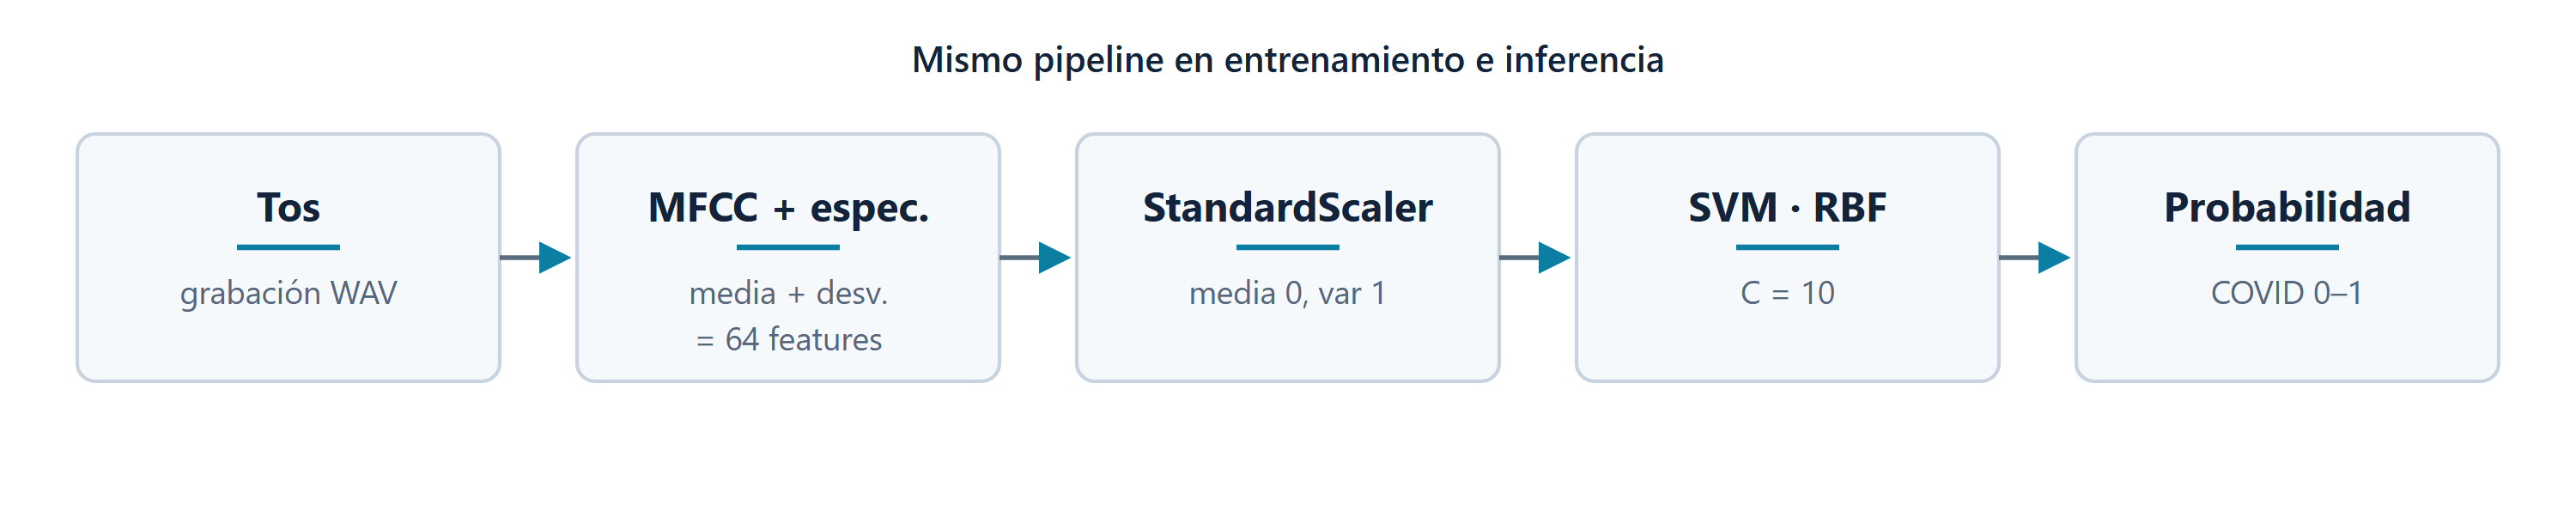
\includegraphics[width=\columnwidth]{figures/pipeline_despliegue.png}}
\caption{Flujo de extracci\'on de caracter\'isticas y predicci\'on, id\'entico en el entrenamiento y en la inferencia en tiempo real. La aplicaci\'on web reutiliza el mismo c\'odigo, por lo que las predicciones desplegadas coinciden con las del estudio.}
\label{fig:despliegue}
\end{figure}
Para poner el modelo en pr\'actica se desarroll\'o una aplicaci\'on web progresiva que permite grabar una tos desde el navegador y obtener una estimaci\'on en tiempo real. El servidor, implementado con FastAPI, reutiliza exactamente el mismo flujo de extracci\'on de caracter\'isticas (\texttt{librosa}) y el mismo modelo (\texttt{scikit-learn}) de los experimentos; por ello las caracter\'isticas y las predicciones coinciden con las reportadas, sin desajuste entre el an\'alisis y el despliegue (Fig.~\ref{fig:despliegue}). La aplicaci\'on incorpora una comprobaci\'on de energ\'ia que descarta grabaciones sin tos y, con consentimiento expl\'icito del usuario, almacena las grabaciones de forma an\'onima para ampliar progresivamente el conjunto de datos, atendiendo a la principal limitaci\'on identificada: la escasez de ejemplos positivos. La herramienta es de car\'acter educativo y no constituye un diagn\'ostico; se encuentra disponible p\'ublicamente\footnote{\url{https://ml-project-classification.onrender.com}}. La arquitectura completa del sistema y el pipeline detallado se documentan en l\'inea\footnote{\url{https://erosas-utec.github.io/ml-project-classification/}}.

\section{Conclusiones}
Se compararon cuatro modelos cl\'asicos de clasificaci\'on, m\'as Random Forest, para detectar COVID-19 a partir del sonido de la tos, empleando caracter\'isticas MFCC y validaci\'on cruzada a nivel de paciente. El mejor modelo fue una SVM con kernel RBF. Se confirm\'o que, bajo un fuerte desbalance de clases, la exactitud es una m\'etrica enga\~nosa y que conviene guiarse por el F1 y el recall de la clase positiva.

De las estrategias de mejora estudiadas, la reducci\'on de dimensionalidad, la ponderaci\'on de clases y los deltas de MFCC no aportaron mejoras en validaci\'on cruzada, mientras que el ajuste del umbral de decisi\'on s\'i mejor\'o de forma consistente la detecci\'on de positivos, con una p\'erdida m\'inima de exactitud global. El principal factor limitante es el desbalance del conjunto y el uso exclusivo del sonido; como trabajo futuro, disponer de m\'as grabaciones positivas o incorporar informaci\'on ac\'ustica adicional podr\'ia mejorar los resultados. Con ese prop\'osito, la aplicaci\'on web desarrollada recolecta nuevas grabaciones con consentimiento. Todo el proyecto emplea una semilla fija (\texttt{SEED = 42}) y separa los conjuntos a nivel de paciente, por lo que los resultados son reproducibles. El c\'odigo fuente completo, incluido el notebook, est\'a disponible en el repositorio p\'ublico \url{https://github.com/erosas-utec/ml-project-classification}.

\begin{thebibliography}{00}
\bibitem{coswara} N. Sharma \emph{et al.}, ``Coswara --- A database of breathing, cough, and voice sounds for COVID-19 diagnosis,'' en \emph{Proc. INTERSPEECH}, 2020, pp. 4811--4815.
\bibitem{virufy} G. Chaudhari \emph{et al.}, ``Virufy: Global applicability of crowdsourced and clinical datasets for AI detection of COVID-19 from cough,'' \emph{arXiv:2011.13320}, 2020.
\bibitem{mfcc} S. Davis y P. Mermelstein, ``Comparison of parametric representations for monosyllabic word recognition in continuously spoken sentences,'' \emph{IEEE Trans. Acoust., Speech, Signal Process.}, vol. 28, n.\textordmasculine{} 4, pp. 357--366, 1980.
\bibitem{librosa} B. McFee \emph{et al.}, ``librosa: Audio and music signal analysis in Python,'' en \emph{Proc. 14th Python in Science Conf.}, 2015, pp. 18--25.
\bibitem{scikit} F. Pedregosa \emph{et al.}, ``Scikit-learn: Machine learning in Python,'' \emph{J. Mach. Learn. Res.}, vol. 12, pp. 2825--2830, 2011.
\bibitem{svm} C. Cortes y V. Vapnik, ``Support-vector networks,'' \emph{Machine Learning}, vol. 20, n.\textordmasculine{} 3, pp. 273--297, 1995.
\end{thebibliography}

\end{document}
